\chapter{Herramienta propuesta}

    El objetivo de esta tesis es el desarrollo de una herramienta que realice automáticamente tanto el diseño del señalamiento como la implementación del sistema de enclavamiento en una plataforma electrónica. El flujo de trabajo mostrado en la Figura \ref{fig:workflow} introduce el Analizador de Redes Ferroviarias (RNA, del inglés, Railway Network Analyzer) y el Generador Automático de Código (ACG, del inglés, Automatic Code Generator). Cada flecha indica las dependencias entre los diferentes bloques. El RNA se enfoca principalmente en el comportamiento estático del sistema, mientras que el ACG se enfoca en el comportamiento dinámico. Ambos son explicados a profundidad en la Sección \ref{sec:RNA} y Sección \ref{sec:ACG} respectivamente.

    \begin{figure}[h]
        \centering
        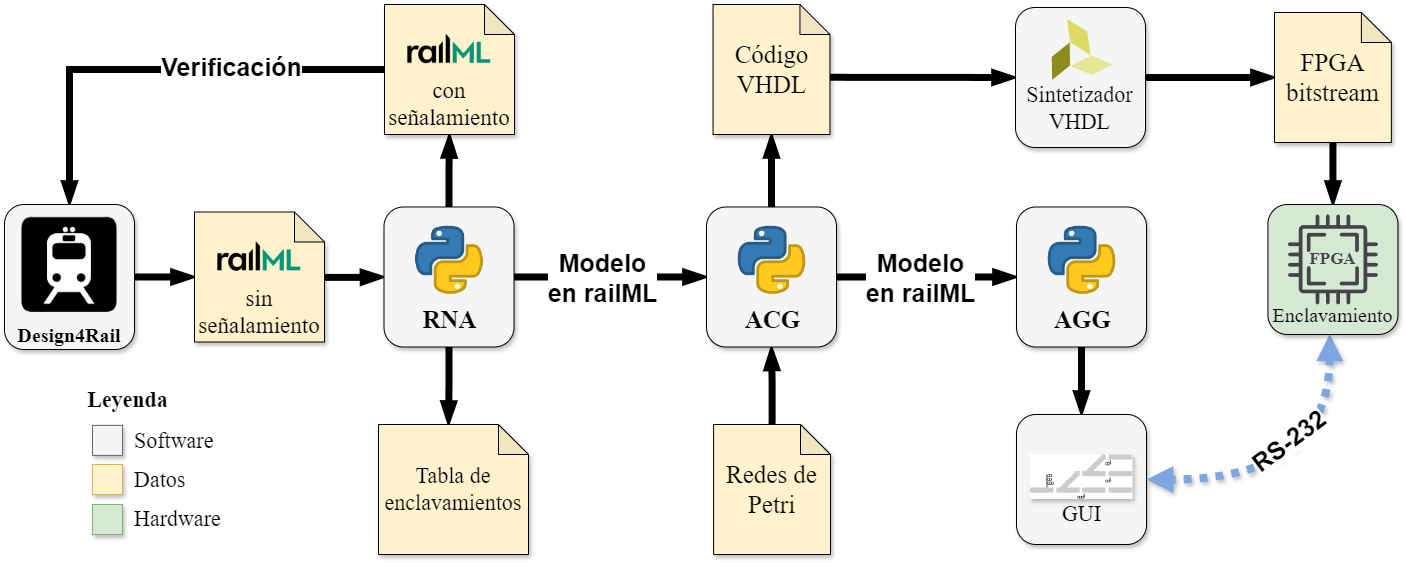
\includegraphics[width=1\textwidth]{Figuras/workflow.png}
        \centering\caption{Flujo de trabajo de la presente tesis.}
        \label{fig:workflow}
    \end{figure}

    El RNA importa un archivo en formato railML que describe el sistema, con o sin señalamiento previo. Luego el RNA analiza la topología de la red, detecta todos los elementos ferroviarios involucrados y genera el señalamiento necesario para que la red sea segura. Finalmente, el RNA exporta un nuevo archivo en formato railML con el nuevo señalamiento, además de la tabla de enclavamientos del sistema, con todas las rutas soportadas por esa red ferroviaria. El nuevo archivo railML es utilizado por el ACG para generar código en VHDL [VHDL] automáticamente para ser sintetizado en una plataforma FPGA [FPGA].
    
    El proceso de validación incluye la validación de la sintaxis del archivo railML generado por RNA, la validación de la tabla de enclavamiento generada automáticamente por RNA y, finalmente, la validación del señalamiento generado conforme a los principios de señalamiento (Sección \ref{sec:principios}). Para implementar automáticamente un sistema de enclavamiento, el ACG toma este diseño de señalamiento estático generado automáticamente y un modelo de comportamiento dinámico en redes de Petri. %Un ingeniero de señalamiento puede realizar un análisis dinámico adicional, incluyendo cualquier problema relacionado con el tiempo, como fallas o retrasos, que están más allá del alcance de este artículo.
    


\section{Enfoque aplicado}

    Durante la Maestría en Sistemas Embebidos se desarrollo un primer prototipo del ACG en base a un rudimentario modelo de redes de grafos. Fue este modelo de grafos el que permitió probar el ACG con una amplia variedad de topologías fácilmente, debido a la flexibilidad, linealidad y escalabilidad del modelo. En esta etapa temprana del proyecto ya se había adoptado un enfoque geográfico.

    La única desventaja de la elección temprana de un enfoque geográfico fue la, aparente, inexistencia de herramientas o soportes formales, para lo cual era necesario desarrollar todo desde cero sin un estándar que lo sostenga. Aún así, una vez desarrollada la herramienta se podía reutilizar las veces necesarias, por lo que las ventajas a largo plazo eran mayores. Al descubrir la existencia de railML, rápidamente se comenzó la migración del ACG para ser compatible con el estándar.

    El desarrollo del RNA, siendo posterior al ACG y a la incorporación de railML, fue completamente en línea con el estándar desde un inicio. Al ser compatibles con railML, tanto el RNA como el ACG deben ser compatibles también con el modelo planteado por RailTopomodel. Debido a esto, el desarrollo de la herramienta deberá seguir indefectiblemente los lineamientos de un enfoque geográfico. 
\section{Arquitectura del sistema}

    \lipsum[1]
\section{Caracteristicas del sistema}

    \lipsum[1]
\section{Validación del sistema}

    Para asegurar la validez de nuestro enfoque, analizamos tanto la validez interna como la externa. En cuanto a la validez interna, es importante garantizar una relación causal entre el diseño proporcionado y la señalización generada sin que ningún otro factor externo afecte el resultado. Podemos aprovechar el hecho de que el modelo ferroviario que el RNA utiliza es un sistema lineal debido a que el RNA se basa en redes de grafos y las redes de grafos son sistemas lineales. De esta manera, las señales generadas para dos elementos ferroviarios A y B serían las mismas que las señales generadas para el elemento ferroviario A más las señales generadas para el elemento ferroviario B. Este análisis se puede extender a cualquier número de elementos ferroviarios diferentes. Esto puede provocar solapamientos de señales, por lo tanto, se añade la posibilidad de que los usuarios de la herramienta habiliten o deshabiliten la simplificación, así como establecer la distancia mínima entre elementos para considerar si se superponen o no.

    Los usuarios pueden seleccionar qué elementos ferroviarios se analizarán. La elección de los elementos a analizar es extremadamente poderosa porque nos permite probar la generación de señales para cada elemento ferroviario individualmente para verificar que se estén analizando correctamente. Una vez que esta verificación se realiza para cada elemento y se confirma que no hay factores externos que afecten la señalización generada, podemos seleccionarlos simultáneamente, sin simplificación. De esta manera, la linealidad del sistema se manifestará por sí misma y, en algunos casos, también la necesidad de simplificación de la señalización (ver Sección \label{sec:simplificacion}). Debido a la linealidad, los elementos ferroviarios que están muy cerca uno del otro se pueden considerar como un solo elemento, lo que resulta en una nueva señalización que tendría menos señales que la suma de sus señales anteriores debido a la simplificación de señales redundantes.

    Respecto a la demostración formal de los resultados, los estudios académicos (ver Sección \ref{sec:estudios}) suelen depender en su mayoría de métodos formales para verificar y validar sus diseños [VV\_4]. Sin embargo, el RNA se basa en redes de grafos y, según la norma IEC 61508 [IEC], las redes de grafos son un método semi-formal. Además, casi la mitad de los estudios respaldados por las empresas mas importantes de la industria ferroviaria utilizan técnicas semi-formales [VV\_4] para reducir la brecha entre la formalidad académica y las necesidades de la industria. Con el fin de realizar pruebas en sistemas ferroviarios reales, damos mayor énfasis a la validación de un enfoque más práctico y menos formal, de acuerdo con los requisitos y tendencias de la industria ferroviaria.
    
    Adicionalmente a la validación del resultado, es importante verificar que el archivo railML generado sea sintácticamente correcto según los estándares de railML. El RNA realiza verificaciones de sintaxis tanto al importar el archivo en formato railML como al generar uno nuevo. Esto se puede confirmar fácilmente importando el archivo railML en Design4Rail [RAILAID], una herramienta certificada por railML.org. Esta herramienta realiza una validación de sintaxis de terceros de nuestros archivos railML generados y también se utiliza para visualizar los diseños ferroviarios generados automáticamente.

    En cuanto a la validez externa, la inclusión de ocho diseños ferroviarios cuidadosamente seleccionados presentados en la Sección XXX tiene como objetivo cubrir una amplia gama de topologías y un uso extensivo de los elementos ferroviarios más comunes. Cuatro de estos ejemplos son diseños reales de ferrocarriles y los otros cuatro se crearon para introducir topologías que se utilizan ampliamente en muchos países. Por lo tanto, cualquier otro diseño ferroviario compartiría la mayoría de las características y elementos modelados en nuestros ejemplos. Si se detecta un nuevo elemento en el diseño, se consideraría como un elemento a proteger y RNA generará la señalización adecuada de acuerdo con los principios P3 y P6 explicados en la Sección \ref{sec:principios}.

    Nuestro proceso de validación implica una comparación automática entre las tablas de enclavamiento aprobadas por las autoridades ferroviarias y las tablas generadas por RNA. La ruta definida por RNA (o conjunto de rutas) debe tener una ruta correspondiente en el diseño original de señalización. Cualquier ruta no definida originalmente debe mejorar la seguridad general al proteger la infraestructura ferroviaria que no se consideró originalmente o mejorar la logística al agregar nuevas rutas no conflictivas. RNA también realiza una validación de sintaxis del archivo railML, indicando si alguna parte de la estructura XML está ausente o dañada. Finalmente, verificamos que todos los principios de señalización introducidos en este artículo sean cumplidos por la señalización generada por RNA mediante un proceso de análisis posterior del diseño y la nueva señalización, asegurando que se cumpla cada principio de diseño ferroviario.